\chapter{Evaluation\label{cha:chapter6}}
This chapter structures in two parts. First, risks and tradeoffs of the concept and implementation are illuminated with an established SOA evaluation method. Second, RG is discussed and possible improvements are pointed out.

\section{The ATAM Method}
\epigraph{It is better to be vaguely right than exactly wrong.}{Carveth Read (1848 – 1931) philosopher and logician}
In this chapter, an excerpt of the architecture tradeoff analysis method (ATAM,~\cite{Kazman1998TheMethod}) as conducted in~\cite{Bianco2007EvaluatingArchitecture} shall be used to evaluate the current implementation and underlying concept. ATAM is a method aimed at illuminating risks in the architecture through the identification of attribute trends, rather than at precise characterizations of measurable quality attribute values~\cite{Kazman1999ExperienceAnalysis}. ATAM focuses on the analysis of quality attributes. Quality attributes, also known as \textbf{nonfunctional requirements}, include usability, performance, scalability, reliability, security and modifiability. Subsection~\ref{subseb:qualatt} provides some generic examples. Subsections~\ref{subsec:atamsteps} and~\ref{subsec:atamgoa} introduce the necessary ATAM steps and the goal of finding risks and tradeoffs. For the introduced framework it is an applicable method as it stays high level. Once it is implemented in an industrial environment, a more quantifiable method is necessary.  

ATAM has been introduced by Kazman in 1998 at Carnegie Mellon University in Pennsylvania~\cite{Kazman1998TheMethod}. It was used on at least 18 architectures in the 2000s~\cite{Bass2007RiskEvaluations}. In 2013, Zalewski introduced an updated ATAM method which can be applied at an even earlier stage of architecture evaluation~\cite{Zalewski2013BeyondSystems}.

\subsection{Quality Attributes}
\label{subseb:qualatt}
The following example quality attributes are decorated with generic examples which are directly quoted from Appendix A in \textit{Evaluating a Service-Oriented Architecture}~\cite{Bianco2007EvaluatingArchitecture}.
\subsubsection{Performance}
\begin{itemize}
    \item A sporadic request for service ‘X’ is received by the server during normal operation. The system processes the request in less than ‘Y’ seconds. 
    \item The service provider can process up to ‘X’ simultaneous requests during normal operation, keeping the response time on the server less than ‘Y’ seconds.  
    \item The roundtrip time for a request from a service user in the local network to service ‘X’ during normal operation is less than ‘Y’ seconds. 
\end{itemize}

\subsubsection{Availability}
\begin{itemize}
    \item An improperly formatted message is received by a system during normal operation. The 
system records the message and continues to operate normally without any downtime. 
    \item An unusually high number of suspect service requests are detected (denial-of-service attack), and the system is overloaded. The system logs the suspect requests, notifies the system administrators, and continues to operate normally. 
    \item Unscheduled server maintenance is required on server ‘X.’ The system remains operational in degraded mode for the duration of the maintenance. 
    \item A service request is processed according to its specification for at least 99.99\,\% of all requests. 
    \item A new service is deployed without impacting the operations of the system. 
    \item A third-party service provider is unavailable; modules that use that service respond appropriately regarding the unavailability of the external service; and the system continues to operate without failures.
\end{itemize}

\subsubsection{Security}
\begin{itemize}
    \item A third-party service with malicious code is used by the system. The third-party service is unable to access data or interfere with the operation of the system. The system notifies the system administrators. 
    \item An attack is launched attempting to access confidential customer data. The attacker is not able to break the encryption used in all the hops of the communication and where the data is persisted. The system logs the event and notifies the system administrators. 
    \item A request needs to be sent to a third-party service provider, but the provider’s identity can not be validated. The system does not make the service request and logs all relevant information. The third party is notified along with the system administrator. 
\end{itemize}

\subsubsection{Testability}
\begin{itemize}
    \item An integration tester performs integration tests on a new version of a service that provides an interface for observing output. 90\,\% path coverage is achieved within one person-week. 
\end{itemize}

\subsubsection{Interoperability}
\begin{itemize}
    \item A new business partner that uses platform ‘X’ is able to implement a service user module that works with our available services in platform ‘Y’ in two person-days.  
    \item A transaction of a legacy system running on platform ‘X’ is made available as a web service to an enterprise application that is being developed for platform ‘Y’ using the web services technology. The wrapping of the legacy operation as a service with proper security verification, transaction management, and exception handling is done in 10 person-days. 
\end{itemize}

\subsubsection{Modifiability}
\begin{itemize}
    \item A service provider changes the service implementation, but the syntax and the semantics of the interface do not change. This change does not affect the service users. 
    \item A service provider changes the interface syntax of a service that is publicly available. The old version of the service is maintained for 12 months, and existing service users are not affected within that period.  
    \item A service user is looking for a service. A suitable service is found that contains no more than ‘X’ percentage of unneeded operations, so the probability of the service provider changing is reduced. 
\end{itemize}

\subsubsection{Reliability}
\begin{itemize}
    \item A sudden failure occurs in the runtime environment of a service provider. After recovery, all transactions are completed or rolled back as appropriate, so the system maintains uncorrupted, persistent data. 
    \item A service becomes unavailable during normal operation. The system detects and restores the service within two minutes. 
\end{itemize}

\subsection{ATAM Steps}
\label{subsec:atamsteps}
ATAM consists of the following steps (directly quoted from~\cite{Bianco2007EvaluatingArchitecture}):
\begin{enumerate}
    \item Present the ATAM: The evaluation team presents a quick overview of the ATAM steps, the techniques used, and the outputs from the process. 
    \item Present the business drivers: The system manager briefly presents the business drivers and context for the architecture.
    \item Present the architecture: The architect presents an overview of the architecture.
    \item Identify architectural approaches: The evaluation team and the architect itemize the architectural approaches discovered in the previous step. 
    \item Generate the quality attribute utility tree: A small group of technically oriented stakeholders identifies, prioritizes, and refines the most important quality attribute goals in a utility tree format.
    \item Analyze the architectural approaches: The evaluation team probes the architectural approaches in light of the quality attributes to identify risks, non-risks, and tradeoffs. 
    \item Brainstorm and prioritize scenarios: A larger and more diverse group of stakeholders creates scenarios that represent their various interests. Then the group votes to prioritize the scenarios based on their relative importance. 
    \item Analyze architectural approaches: The evaluation team continues to identify risks and tradeoffs while noting the impact of each scenario on the architectural approaches. 
    \item Present results: The evaluation team recapitulates the ATAM steps, outputs, and recommendations.
\end{enumerate}

These steps are typically carried out in two phases. Phase~1 is architect-centric and concentrates on eliciting and analyzing architectural information. This phase includes a small group of technically oriented stakeholders concentrating on Steps~1 to~6. Phase~2 is stakeholder-centric, elicits points of view from a more diverse group of stakeholders, and verifies the results of the first phase. This phase involves a larger group of stakeholders, builds on the work of the first phase, and focuses on Steps~7 through~9.~\cite{Jones2001EvaluateStudy} 

\subsection{ATAM Goals}
\label{subsec:atamgoa}
It is desired to find risks and tradeoffs:
\begin{itemize}
    \item risks: architectural decisions that might create future problems for some quality attribute. A sample risk: The current version of the Database Management System is no longer supported by the vendor; therefore, no patches for security vulnerabilities will be created.
    \item tradeoffs: architectural decisions that have an effect on more than one quality attribute.     For example, the decision to introduce concurrency improves latency but increases the cost of change for the affected modules. 
\end{itemize}

\section{Architecture Evaluation of RG with ATAM Method}
In this evaluation chapter, I will cover steps 7 and 8 as described in subsection~\ref{subsec:atamsteps}. As a goal, I will identify risks and tradeoffs. The list is claimed to be incomplete and just covers some important aspects that were considered during service design. Also, in practice, ATAM can be iterated which is dropped here.

\subsection{Quality Attribute Scenarios}
For an explanaition of the sources (i.e., roles), see annex~\ref{sec:involvedparties}.
TODO evtl die abbildung in den anhang und die wichtigsten punkte textuell beschreiben
{\renewcommand{\arraystretch}{0.7} % vertical spacing between rows
\begin{longtable}{|P{0.08\linewidth}|P{0.2\linewidth}|P{0.16\linewidth} P{0.44\linewidth}|}
\caption{Quality Attribute Scenarios}\label{tab:scen}\\
\hline
\rowcolor{Gray}
\textbf{Number} & \textbf{Quality Attribute} & \multicolumn{2}{l|}{\textbf{Scenario}}\\
\hline
\endfirsthead
\multicolumn{4}{c}%
{\tablename\ \thetable\ -- \textit{Continued}} \\
\hline
\rowcolor{Gray}
\textbf{Number} & \textbf{Quality Attribute} & \multicolumn{2}{l|}{\textbf{Scenario}}\\
\hline
\endhead
\hline \multicolumn{4}{r}{\textit{Continued on next page}} \\
\endfoot
\hline
\endlastfoot
 1 & Modifiability & Source:  & Detector Docker Image Provider\\
   & & Stimulus:  & Add a new detector\\ 
   & & Artifact:  &  Docker Registry \\ 
   & & Environment:  & Detector provider familiar with Docker, gRPC and detector proto file\\ 
   & & Response:  & New detector is added\\ 
   & & Response Measure:  & No more than five person-days of detector provider team effort is required for the implementation (legal and financial agreements are not included).\\ \hline 
 2 & Modifiability & Source:  & Camera Docker Image Provider\\
   & & Stimulus:  & Add a new camera to the vision system\\ 
   & & Artifact:  &  Camera \\ 
   & & Environment:  & Camera provider familiar with Docker, gRPC and camera proto file\\ 
   & & Response:  & New camera is added\\ 
   & & Response Measure:  & No more than four person-days of camera provider team effort is required for the implementation (legal and financial agreements are not included).\\ \hline
 3 & Modifiability & Source:  & RG Client\\
   & & Stimulus:  & Add a new proto file version\\ 
   & & Artifact:  &  Camera or Detector \\ 
   & & Environment:  & A new version of a proto file is necessary due to missing message types\\ 
   & & Response:  & New proto file is added\\ 
   & & Response Measure:  & No more than one person-day of effort is necessary. All existing camera and detector service remain functional.\\ \hline
 4 & Interoperability & Source  & Framework Architect\\
   & & Stimulus:  & Replace or scratch Docker\\ 
   & & Artifact:  & Detector and Camera Image Docker Containers\\ 
   & & Environment:  & Docker is not allowed or not possible to use\\ 
   & & Response:  & Docker is replaced or scratched\\ 
   & & Response Measure:  & No more than fifteen person-days of framework architect effort is required for the implementation\\ \hline
 5 & Performance & Source  & Detector Docker Image Provider\\
   & & Stimulus:  & Send a file to detector\\ 
   & & Artifact:  & Detector Docker Container\\ 
   & & Environment:  & CAD file input not larger than 10\,MB sent to detector\\ 
   & & Response: & File to detector sent\\ 
   & & Response Measure:  & The trip time for a request from detector client in the local network to detector during normal operation is less than 2 seconds.\\ \hline
 6 & Reliability & Source  & Framework Architect\\
   & & Stimulus  & Service failure\\ 
   & & Artifact  & All components\\ 
   & & Environment  & A sudden failure occurs in the runtime environment of a service.  \\ 
   & & Response  & After recovery, all transactions are completed or rolled back as appropriate, so the system maintains uncorrupted, persistent data.\\ 
   & & Response Measure:  & Manual test if data is corrupt or inconsistent.\\ \hline
 7 & Security & Source  & A possible attacker\\
   & & Stimulus  & A malware is included in the system\\ 
   & & Artifact  & Camera or Detector Docker Container\\ 
   & & Environment  & We have to face a denial-of-service attack.  \\ 
   & & Response  & The malware is detected quickly, best before entering the framework. Necessary information to possibly identify the attacker is logged.\\ 
   & & Response Measure:  & Our system is not operable for not more than an hour.\\ \hline
\end{longtable}
\newpage
\subsection{Architectural Analysis of Scenarios}
TODO evtl die abbildung in den anhang und die wichtigsten punkte textuell beschreiben
\begin{longtable}{| P{0.2\textwidth} | P{0.74\textwidth} |}
\caption{Architectural Analysis of Scenarios}\label{tab:scenan}\\
\hline
\endfirsthead
\multicolumn{2}{c}%
{\tablename\ \thetable\ -- \textit{Continued}} \\
\hline
\endhead
\hline \multicolumn{2}{r}{\textit{Continued on next page}} \\
\endfoot
\hline
\endlastfoot
\rowcolor{Gray}
\multicolumn{2}{ |l| }{\textbf{Analysis for Scenario 1}} \\ \hline
Scenario Summary & New Detector added to Docker Registry in no more than five person-days\\ \hline
Business Goal(s) & Extending the available object detection possibilities\\ \hline
Quality Attribute & Modifiability\\ \hline
Architectural Approaches and Reasoning & Detector communication depends on gRPC which covers many programming languages and a REST gateway. \newline Docker registry can be made easily accessible for the provider and is a well-known technology.\\ \hline
Risks &  Possible too much of a lock-in effect of both technologies\\ \hline
Tradeoffs &  The static Train/Test interface might not (yet) be suitable for all detection purposes, although once implemented it is very easy to use and might become more popular as a versioned standard.\\ \hline
\rowcolor{Gray}
\multicolumn{2}{ |l| }{\textbf{Analysis for Scenario 2}} \\ \hline
Scenario Summary & New camera added to vision system in no more than four person-days\\ \hline
Business Goal(s) & Possibility of heterogeneous camera ecosystem\\ \hline
Quality Attribute & Modifiability\\ \hline
Architectural Approaches and Reasoning & Docker container including or alternatively just gRPC server running on camera which allows for many programming languages \\ \hline
Risks &  The camera firmware can be unmodifiable, thus a middleware is likely to be needed. \\ \hline
Tradeoffs & In theory, the same underlying technology (Docker + gRPC) can be conveniently used for communication between recipe and camera, but in practice, at least for the camera, this might end up cumbersome without a fitting middleware. \\ \hline
\rowcolor{Gray}
\multicolumn{2}{ |l| }{\textbf{Analysis for Scenario 3}} \\ \hline
Scenario Summary & A new proto file version is added in no more than on person-day.\\ \hline
Business Goal(s) & Staying up to date with current ODMs\\ \hline
Quality Attribute & Modifiability\\ \hline
Architectural Approaches and Reasoning & gRPC offers a convenient way of expanding proto files. As long as no messages are deleted or overwritten, the system remains downward compatible.\\ \hline
Risks &  None\\ \hline
Tradeoffs &  The more messages are created, the more overhead will be sent over the channels.\\ \hline
\rowcolor{Gray}
\multicolumn{2}{ |l| }{\textbf{Analysis for Scenario 4}} \\ \hline
Scenario Summary & Replace or scratch Docker in no more than 15 person-days.\\ \hline
Business Goal(s) & Permit easy integration with new business partners. \\ \hline
Quality Attribute & Interoperability\\ \hline
Architectural Approaches and Reasoning & Detector and Camera gRPC servers/clients do not need Docker for successful communication. It offers a huge convenience for sharing them, starting them, handling dependencies, etc. A switch to e.g. Heroku would require a partial rewrite of the framework.\\ \hline
Risks &  Too much effort included rewriting the framework. Instead, an alternative framework might be used.\\ \hline
Tradeoffs & If Docker is available, the ease of service administration is very high. If not, the flexibility is higher but requires more effort.\\ \hline
\rowcolor{Gray}
\multicolumn{2}{ |l| }{\textbf{Analysis for Scenario 5}} \\ \hline
Scenario Summary & A 10\,MB file is sent to detector in less than 2 seconds. \\ \hline
Business Goal(s) & Compatible message transmission speed.\\ \hline
Quality Attribute & Performance\\ \hline
Architectural Approaches and Reasoning &  gRPC sends its data via protobufs which are a binary format specialized in high-performance serialization and deserialization. If an image has to be transferred between OPC UA Server and Client, then the emerging Time Sensitive Networking will help facing real-time transmission challenges.\\ \hline
Risks & If too slow, the process might the bottleneck in production.\\ \hline
Tradeoffs &  None\\ \hline
\rowcolor{Gray}
\multicolumn{2}{ |l| }{\textbf{Analysis for Scenario 6}} \\ \hline
Scenario Summary & Uncorrupted, persistent data remains on the system after a service failure.\\ \hline
Business Goal(s) & Industrial-grade reliability \\ \hline
Quality Attribute & Reliability\\ \hline
Architectural Approaches and Reasoning & The framework relies on service choreography and client/server communication. Thus, every component has to ensure uncorrupted and persistent data. In the future, a messaging broker could be introduced for better reliability.\\ \hline
Risks & Currently, no reliability is granted, so a service failure will result in a failure of most components of the system \\ \hline
Tradeoffs & Adding a message broker adds reliability but also complexity. \\ \hline
\rowcolor{Gray}
\multicolumn{2}{ |l| }{\textbf{Analysis for Scenario 7}} \\ \hline
Scenario Summary & A denial-of-service attack causes no more than an hour of downtime of the framework.\\ \hline
Business Goal(s) & Offering a secure framework with little downtime. \\ \hline
Quality Attribute & Security\\ \hline
Architectural Approaches and Reasoning & The Docker Hub is intended to be accessible by many vendors to ensure a variety of detectors and cameras. Every new vendor has to ensure its integrity. New detectors and cameras have to be tested thoroughly for a possible malware function. Through the standardized interface, a malfunctioning service can best be replaced quickly by an equivalent one offered by another vendor.\\ \hline
Risks &  A service that is relied on in production reveals itself as malware can be hard to replace in the given time of one hour. Redundant services by multiple vendors can help out in this case.\\ \hline
Tradeoffs & Due to possibly high numbers of services and creative attackers, testing every new vendor and service can be a tedious task.\\ \hline
\end{longtable}
}

\section{Discussion and Possible Improvements}
The discussion of RG is structured in the three sub-tasks of this thesis - generating ODS automatically, handling ODS with varying interfaces and handling ODS with varying ODMs. Although the goals intertwine, they are focused on as separately as possible. Every subsection includes means of possible improvements.

\subsection{Generating Object Detection Services Automatically}
This goal has been reached partly. RG enables the user in composing the necessary services by loading them from the service registry, training the ODS, pushing them back to the registry and finally transferring and executing them. What RG does \textbf{not} do is creating untrained ODM in the first place. Nor does it contain a smart mechanism to choose which ODM is best for a certain OD task which is one of the aspects apart from ODM configuration which requires a high exptertise.

The idea of a future research direction is a device and/or service catalogue. An example for this is the open-source project Eclipse Vorto~\cite{Eclipse2019Vorto2019}. Screenshots are depicted in figures~\ref{fig:vorto} and~\ref{fig:vorto2}. The catalogue helps users describe, share and integrate their services. As the project is community-based, every user can upload content such as cameras, ODMs or data types.

\begin{landscape}
\begin{figure}[ht]
    \centering
    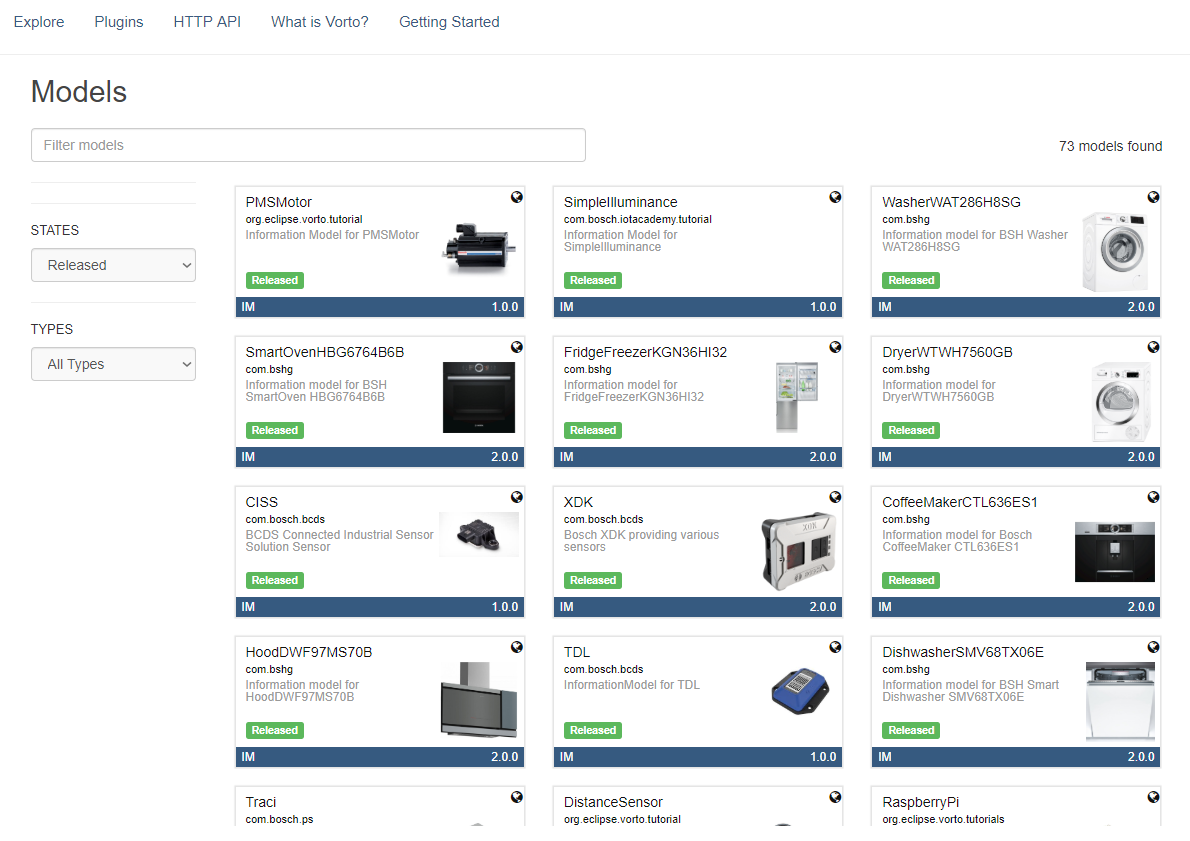
\includegraphics[width=1.3\textwidth]{img/EclipseVorto.png}
    \caption[Eclipse Vorto's device catalogue]{Screenshot of Eclipse Vorto's device catalogue. Every device has a self-explaining interface semantic. The catalogue is community based, i.e. everyone can add his or her device~\cite{Eclipse2019Vorto2019}.}
    \label{fig:vorto}
\end{figure}
\end{landscape}

Choosing an applicable ODM for a specific task can then be handled by the community through a rating system. If the user base is big enough, it will be possible to evaluate best practices for camera/ODM/machine/part type combinations.

Moreover, ODS can provide (hyperlinks to) tutorials and offer workshops alongside the ODS to better scale their know-how. The ODMs or their source code do not have to be revealed with the advantage of a lower incentive to add content to the catalogue.

The challenge for this catalogue is to reach a critical mass (i.e., active users) to prosper.

\begin{figure}[ht]
    \centering
    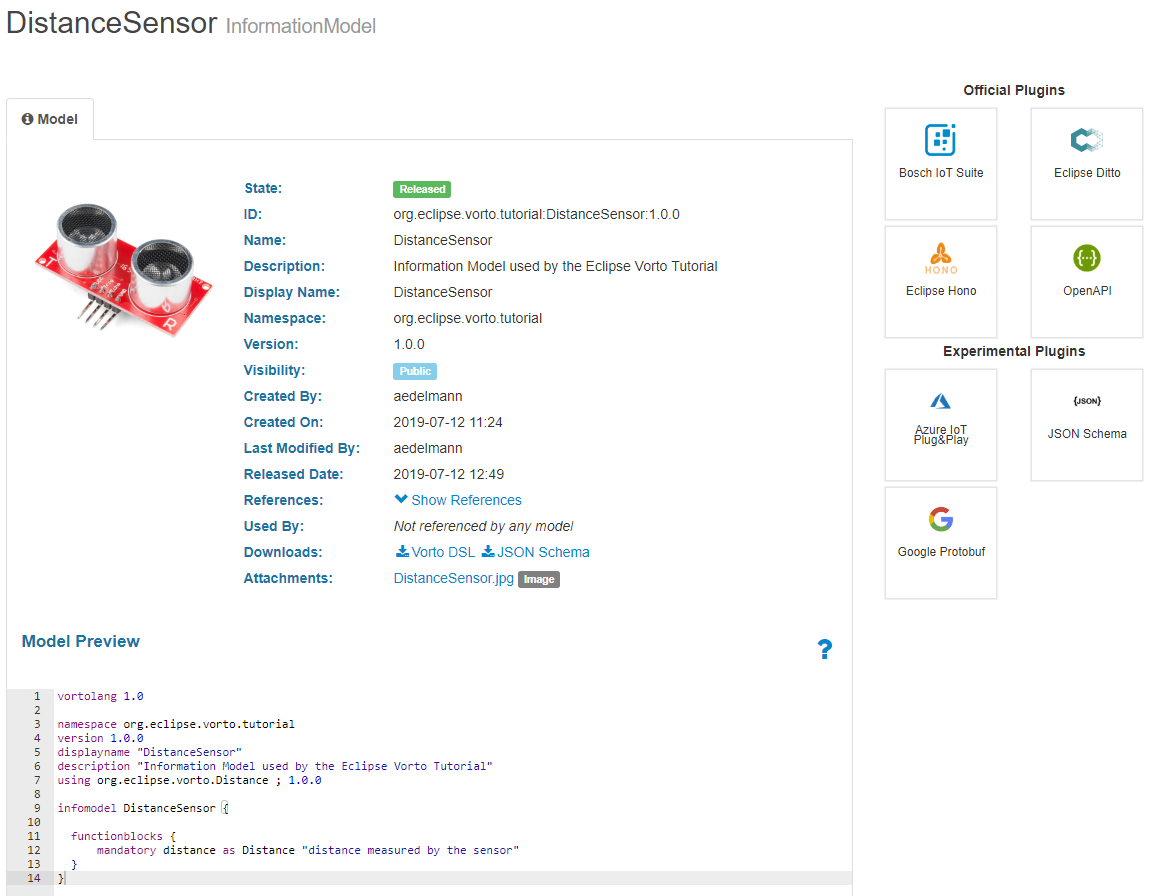
\includegraphics[width=\textwidth]{img/ScreenshotVortoDistanceSensor.png}
    \caption[Distance sensor in Eclipse Vorto's device catalogue]{Screenshot of a detail view of a distance sensor in Eclipse Vorto's device catalogue. Every device has a self-explaining interface semantic. Data types can be shared between devices~\cite{Eclipse2019Vorto2019}.}
    \label{fig:vorto2}
\end{figure}

\subsection{Handling Object Detection Services with Varying Interfaces}
RG uses gRPC for service communication. There is the possibility to offer a REST gateway~\cite{gRPC-Gateway-Documentation2017Grpc-gateway.2018} as well. This covers a broad range of (web-) services. Still, the framework highly depends on the ODS provider and his ODM configurability to interact with RG. Some ODS providers do not offer a gRPC interface. In this case, the REST gateway would also not find a remedy since it only maps REST to gRPC, not vice versa. Hence, for now RG mainly has to work with open-source ODM. Also, the services are dockerized. This is a convenient way of deployment for ODS that the RG user owns. RG does not yet however give possibility to utilize cloud-based pay-per-use ODS like, e.g., Google cloud vision offers~\cite{Google-Cloud-Documentation2019Google2019-04-26}. A REST client would facilitate RG to work with most cloud-based services.
- grpc echtzeitfähig
- andere methode 
- highly dependent of the ODS provider and his ODM configurability
- katalog für devices (vorto) und ODM skizzieren (gelbe seiten)

\subsection{Handling Object Detection Services with Varying Object Detection Methods}
ODS providers need to prepare their method for RG:
- erste abstrahierung mit train und test. besser wäre wenn man sie verschachtelbar macht.
- docker
- eclipse vorto
- services sind schön logisch entkoppelt . kamera muss alerdings drauf geachtet werden, dass service nicht zu sehr auf hardware zugeschnitten ist 
- evtl granularisierung erhöhen innerhalb eines ODS um wiederverwendbarkeit zu erhöhen

- OT --> real-time capabilities of the framework?
    - gRPC specialized for IT, real-time (deterministic, information available exactly when it is needed) is not focused on
    - ODM have to be real-time capable
    - hardware is also not ready yet

TODO    \url{https://vorto.eclipse.org/#/details/org.eclipse.vorto:Acceleration:1.0.0}
    katalog für cameras und odm skizieren
TODO gRPC echtzeitfähig?
TODO Diskussion, Zusammenfassung. Roter Faden! Leser abholen! Die drei Punkte aufgreifen:     Generating ODS automatically
    Handling ODS with varying detection methods
    Handling ODS with varying interfaces
ZUSAMMENFASSUNG https://resources.sei.cmu.edu/library/asset-view.cfm?assetid=513908
The most important results are improved architectures. The output of an ATAM is an outbrief presentation and/or a written report that includes the major findings of the evaluation. These are typically

a set of architectural approaches identified
a "utility tree"—a hierarchic model of the driving architectural requirements
the set of scenarios generated and the subset that were mapped onto the architecture
a set of quality-attribute-specific questions that were applied to the architecture and the responses to these questions
a set of identified risks
a set of identified non-risks
a synthesis of the risks into a set of risk themes that threaten to undermine the business goals for the system

Many people have a stake in a system's architecture, and all of them exert whatever influence they can on the architect(s) to make sure that their goals are addressed. For example, the users want a system that is easy to use and has rich functionality. The maintenance organization wants a system that is easy to modify. The developing organization (as represented by management) wants a system that is easy to build and that will employ the existing work force to good advantage. The customer (who pays the bill) wants the system to be built on time and within budget. All of these stakeholders will benefit from applying the ATAM. And needless to say, the architect is also a primary beneficiary.

